%-------------------------------------------------------------------------------
\newcommand{\toexplain}[1]{
    \textcolor<2>{white}{\textcolor<3>{red}{#1}}
}
\begin{frame}
\createtitle{Research Question}
\begin{center}
\textbf{\large ``\textit{To what extent (and in what manners) does utilizing \toexplain{Transfer Learning} allow \toexplain{Vision Transformers} to perform on par with \toexplain{Convolutional Neural Networks} on common \toexplain{art classification problems}, when compute resources are limited to a single \toexplain{GPU}?}''}
\end{center}
\end{frame}
%-------------------------------------------------------------------------------

%-------------------------------------------------------------------------------
% IT HURTS, but I have to remove this because its too long already D-':
%\begin{frame}
%\createtitle{Transfer Learning}

%\begin{columns}
%\pause
%\column{0.5\textwidth}
%{\large Learning = \textbf{Machine} Learning:}
%\pause
%\begin{itemize}
%\item Data that `summarizes' all previous learning experiences;
%\pause
%\item Way of updating that data with new experiences;
%\pause
%\item Way of making decisions based on that data.
%\pause
%\end{itemize}

%\column{0.5\textwidth}
%But what about Artificial Neural Networks?
%\begin{figure}
%\input{img/ann.pdf_tex}
%\end{figure}

%\end{columns}
%\end{frame}
%-------------------------------------------------------------------------------

%-------------------------------------------------------------------------------
\begin{frame}

\pause
\createtitle{Transfer Learning}
\begin{block}{In this context...}
Learning = \textbf{Machine} Learning
\end{block}

\pause
\begin{columns}[t]
\column{0.5\textwidth}
\centering
Task $T_A$\\
\vspace{0.15cm}
$f($
\raisebox{-0.3cm}{
\includegraphics[width=0.8cm]{img/cat.png}}
$) =$ \texttt{cat}

$f($
\raisebox{-0.3cm}{
\includegraphics[width=0.8cm]{img/dog.png}}
$) =$ \texttt{dog}
\column{0.5\textwidth}
\pause
\centering
Model $M_A$\\
\def\svgwidth{0.5\textwidth}
\input{img/ann.pdf_tex}
\end{columns}

\begin{columns}
\column{0.5\textwidth}
\pause
\centering
Task $T_B$\\
\vspace{0.15cm}
$f($
\raisebox{-0.1cm}{
\includegraphics[width=0.8cm]{img/garfield.jpeg}}
$) =$ \texttt{cat}

$f($
\raisebox{-0.3cm}{
\includegraphics[width=0.8cm]{img/odie.png}}
$) =$ \texttt{dog}
\column{0.5\textwidth}
\pause
\centering
Can we somehow use $M_A$ to improve performance on $T_B$?
\end{columns}

\end{frame}
%-------------------------------------------------------------------------------

%-------------------------------------------------------------------------------
\begin{frame}
\createtitle{Transfer Learning}

\begin{definition}
\textbf{Transfer Learning:} {\footnotesize taking advantage of a model $M_A$ that was trained on task $T_A$ to improve performance on task $T_B$.}
\end{definition}

\pause
\begin{definition}
\textbf{Fine-tuning:} {\footnotesize a type of Transfer Learning where we take $M_A$ as a starting point for training on $T_B$, instead of a newly initialized model.}
\end{definition}

\pause
\begin{definition}
\textbf{Off the shelf learning:} {\footnotesize same as fine-tuning, except that all but the final layer is kept frozen during training.}
\end{definition}

\end{frame}
%-------------------------------------------------------------------------------

%-------------------------------------------------------------------------------
\begin{frame}
\createtitle{Convolutional Neural Networks\\and Vision Transformers}

\pause
Convolutional Neural Networks (CNNs) \tinycite{lecun1998gradient}
\begin{itemize}
\item Have been around for a long time;
\item Played a dominant role in Computer Vision the last decade.
\end{itemize}

\pause
Vision Transformers (VTs) \tinycite{dosovitskiy2020image}
\begin{itemize}
\item Fairly new (2020);
\item Have been taking over in Computer Vision;
\item Based on the Transformer architecture \tinycite{vaswani2017attention}.
\end{itemize}

\end{frame}
%-------------------------------------------------------------------------------

%-------------------------------------------------------------------------------
\begin{frame}
\createtitle{Architecture}

\begin{columns}
\column{0.6\textwidth}
\begin{figure}
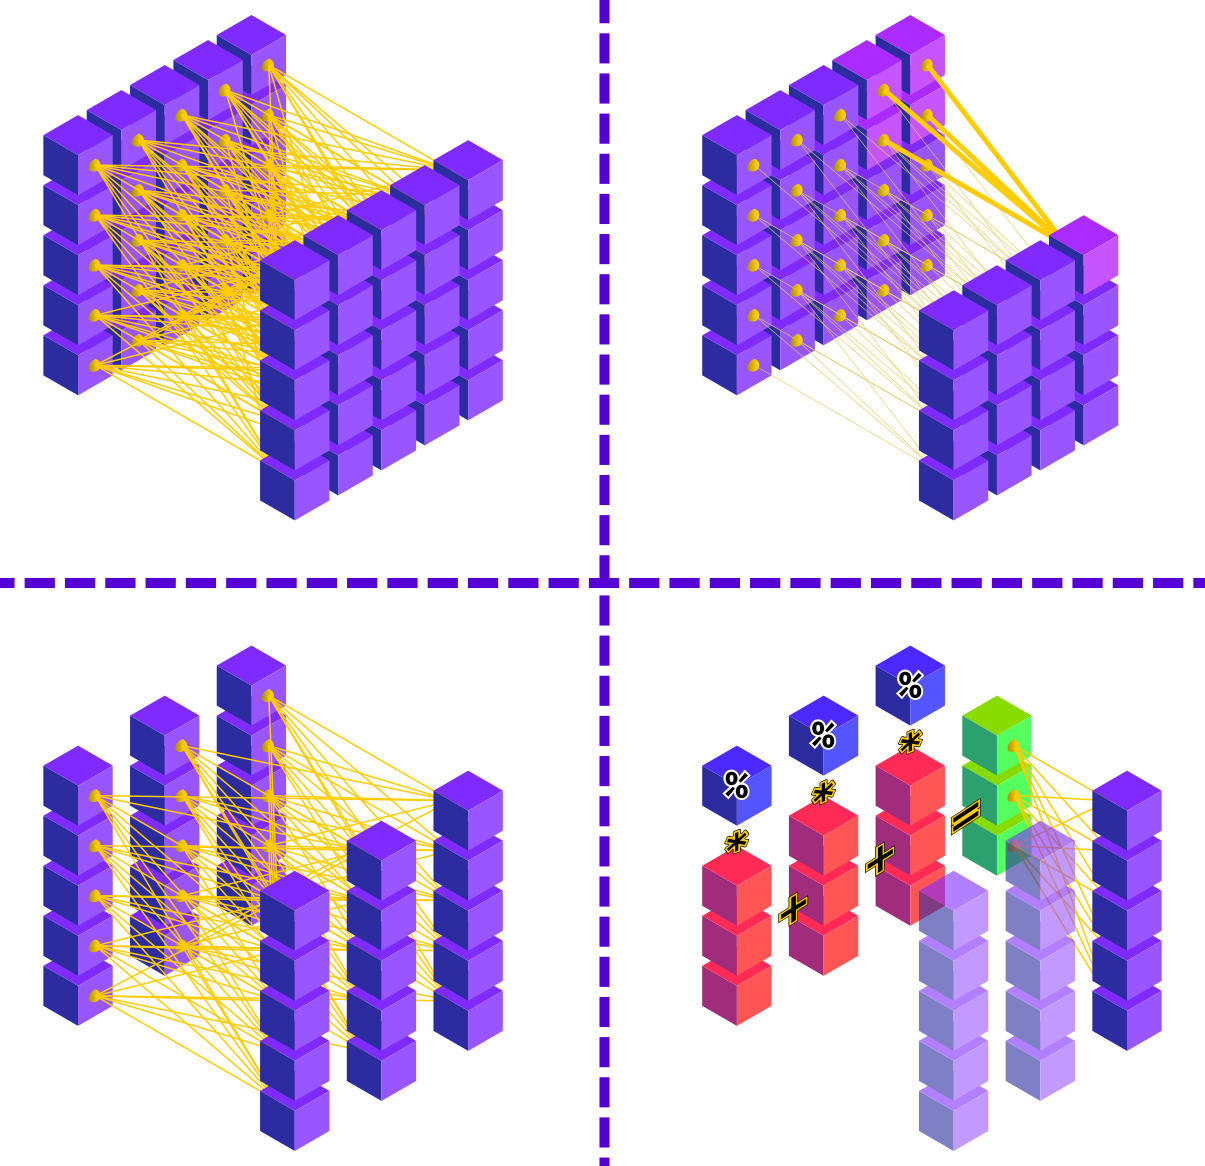
\includegraphics[width=\textwidth]{img/vit_vs_cnn.png}
\caption{\tiny Top right: CNN, Bottom right: Transformer,

Top + Bottom left: hypothetical fully connected variants.}
\end{figure}

\column{0.4\textwidth}
\begin{itemize}
\pause
\item CNNs: designed to work with images;
\pause
\item Transformers (\alert{Not VTs!}): designed for natural language processing.
\end{itemize}

\end{columns}

\end{frame}
%-------------------------------------------------------------------------------

%-------------------------------------------------------------------------------
\begin{frame}
\createtitle{From Transformer to Vision Transformer}

Split image up into $16 \times 16$ patches, and treat them as words in a sentence.
\vspace{0.5cm}

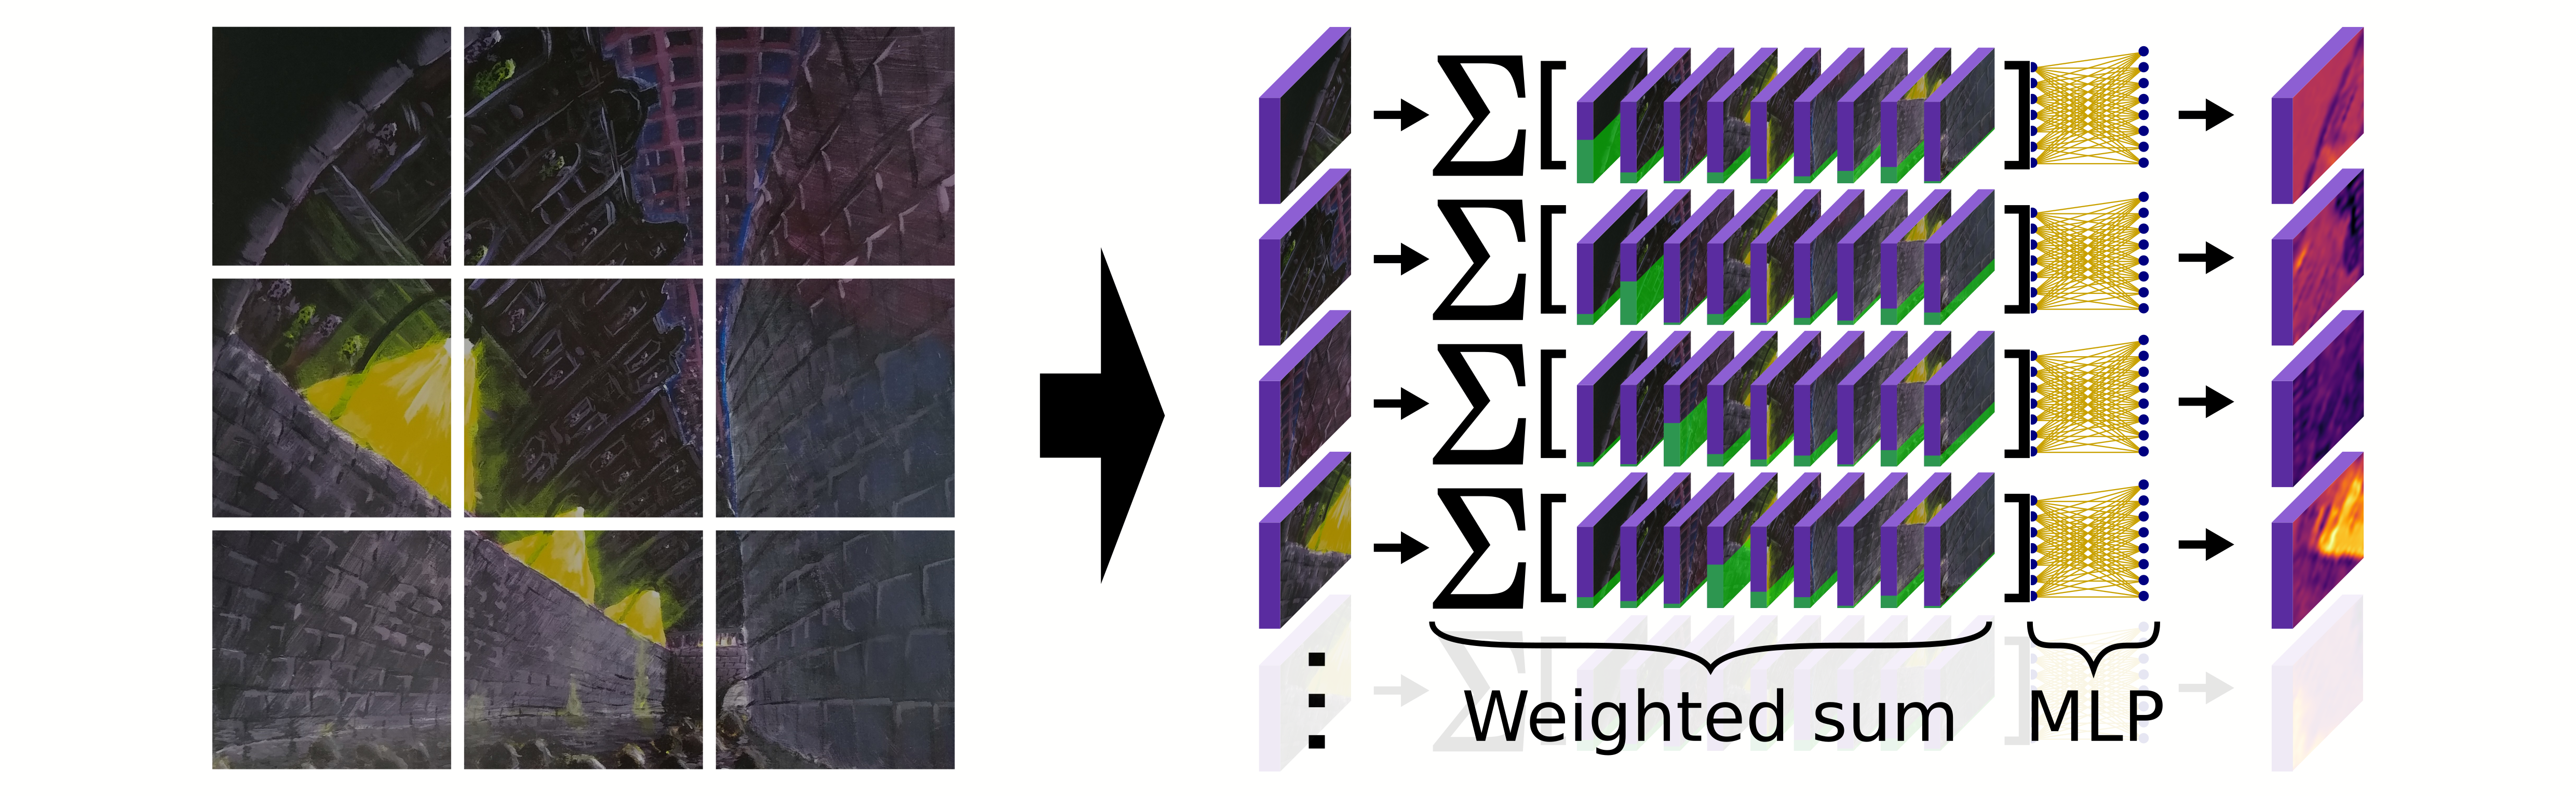
\includegraphics[width=\textwidth]{img/vit_illustration.png}

\pause
\vspace{0.5cm}
Transfer Learning to the rescue!

\end{frame}
%-------------------------------------------------------------------------------

%-------------------------------------------------------------------------------
\newcommand{\stilltoexplain}[1]{\textcolor{red}{#1}}
\begin{frame}
\createtitle{Research Question}
\begin{center}
\textbf{\large ``\textit{To what extent (and in what manners) does utilizing Transfer Learning allow Vision Transformers to perform on par with Convolutional Neural Networks \pause on common \stilltoexplain{art classification problems}, when compute resources are limited to a single \stilltoexplain{GPU}?}''}
\end{center}
\end{frame}
%-------------------------------------------------------------------------------

%-------------------------------------------------------------------------------
\begin{frame}
\createtitle{Art Classification Problems}
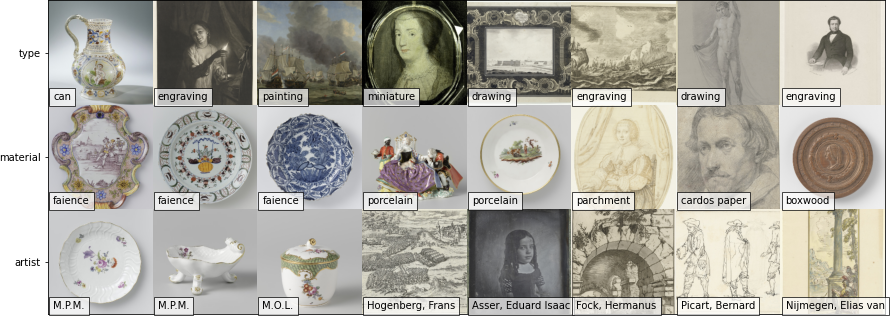
\includegraphics[width=\textwidth]{img/examples.png}

\vspace{0.5cm}
\centering
Taken from ``\textit{The Rijksmuseum Challenge}'' dataset \tinycite{mensink14icmr}.
\end{frame}
%-------------------------------------------------------------------------------

%-------------------------------------------------------------------------------
\begin{frame}
\createtitle{GPU}
\begin{columns}
\column{0.8\textwidth}
Graphics processing unit
\begin{itemize}
\item Does the actual computations.
\end{itemize}
\column{0.2\textwidth}
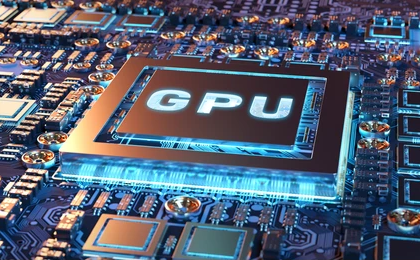
\includegraphics[width=\textwidth]{img/gpu.png}
\end{columns}
\vspace{0.5cm}
\pause
\rule{\textwidth}{0.7pt}

\vspace{0.5cm}

Why this constraint? ...
\pause

\vspace{0.5cm}

... Well, because I am specifically interested in:
\begin{itemize}
\item Problems not too demanding for consumer-grade hardware;
\item Datasets small enough to be labelled by one person.
\end{itemize}
\pause
In other words: focusing on the realm of tinkerers!
\end{frame}
%-------------------------------------------------------------------------------
